\documentclass[20pt, a0paper, landscape,colspace=0.8cm,blockverticalspace=0.8cm,innermargin=0.8cm]{tikzposter}
\title{\centering Bayesian Non-Parametric Inference
                        in Multivariate Peaks-over-Thresholds Models}
\author{Peter Trubey \& Bruno Sans{\'o}}
\date{September 7, 2022}
\institute{UC Santa Cruz; Department of Statistics}

\usepackage{blindtext}
\usepackage{amsmath}
\usepackage{amssymb}
\usepackage{bm}
\usepackage{comment}
\usepackage{nccmath}
\usepackage{booktabs}
\usepackage{enumitem}

\usetheme{Desert}

\begin{document}

\maketitle

\begin{columns}
    \column{0.333}
    \block{Multivariate Peaks-over-Thresholds}{
        For $d$-dimensional random vector $\bm{W} = (W_1,\ldots,W_d) \sim F$;   
        assume the existence of sequences of vectors $\bm{a}_n,\bm{b}_n$ such that 
        \[\lim\limits_{n\to\infty}F^n\left(\bm{a}_n\bm{w} + \bm{b}_n\right) = G(\bm{w}),\] 
        then $G$ is a $d$-variate GEV.  It follows that\\
        \[
        \lim\limits_{n\to\infty}\text{Pr}\left(\frac{\bm{W} - \bm{b}_n}{\bm{a}_n} \leq \bm{w}\mid \bm{W} 
            \not\leq \bm{b}_n\right) = \frac{\log G(\bm{w}\wedge \bm{0}) - \log G(\bm{w})}{\log G(\bm{0})} = H(\bm{w}),
            \]\\
        where $H$ is multivariate Pareto.  In practice, for a sufficiently large
        threshold $\bm{b}$, we model excesses as generalized Pareto.
        
        For ease of interpretation, we transform $W$ to standardized marginals. Let 
        \[Z_{\ell} = \left(1 + \xi_{\ell}\frac{w_{\ell} - b_{\ell}}{a_{\ell}}\right)_+^{1/\xi_{\ell}},\]
        then $\bm{Z}$ follows the standard multivariate Pareto distribution.
        \vspace{1cm}
        \begin{center}
        \begin{tikzfigure}[2-dimensional generalized Pareto (left) transformed to standard marginals (right).]
            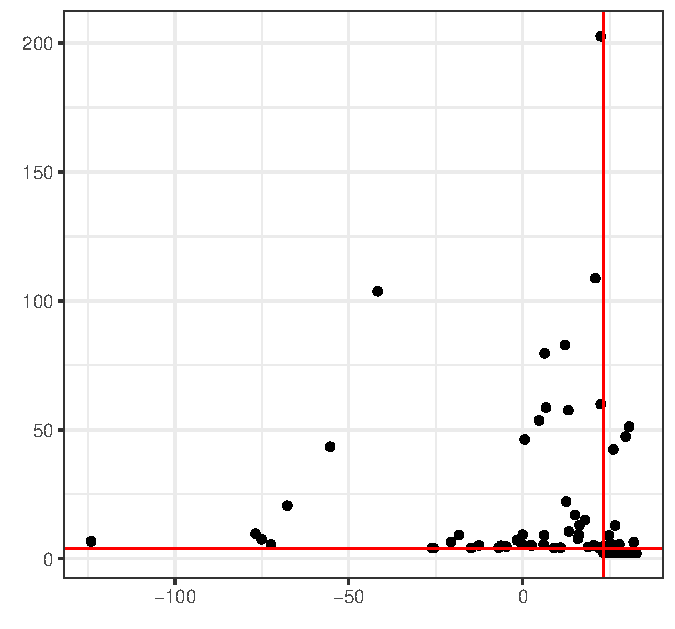
\includegraphics[width=0.12\textwidth]{images/genpareto2d}
            ~
            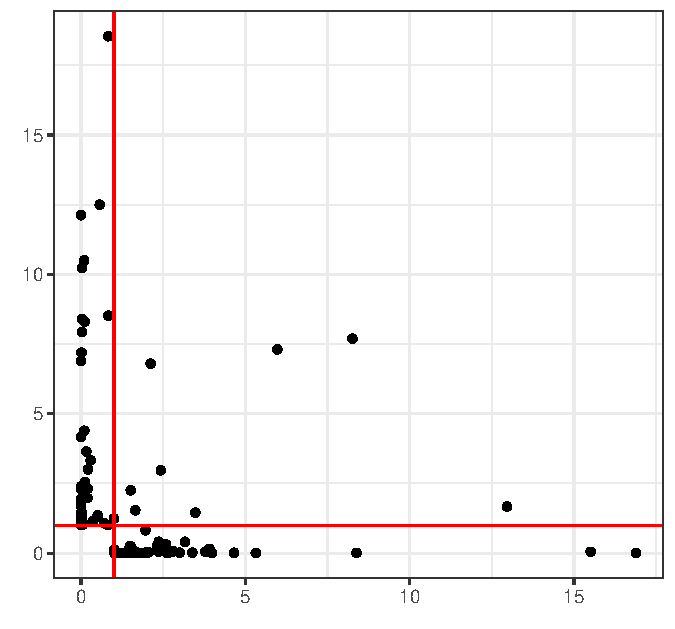
\includegraphics[width=0.12\textwidth]{images/stdpareto2d}
        \end{tikzfigure}
        \end{center}
        
        \vspace{1cm}
        Remark 3.1 of Rootzen et al, 2018 shows how % \cite{rootzen2018} shows how
        we can factorize \[\bm{Z} =
            R\bm{V},\;\;R\in\mathbb{R}_+;\;V\in\mathbb{S}_{\infty}^{d-1},\]
        with $R$ independent of $\bm{V}$. 
        That is, we can factorize $Z$ into
        \emph{independent} angular and radial components. $R$ will follow
        a standard Pareto distribution, and $\bm{V}$ will contain all 
        information related to the dependence structure of $\bm{W}$ in extreme
        regions.  For that reason, we seek a flexible distribution to model
        $\bm{V}$.
        }
    \block{Scoring Criteria for distributions on $\mathbb{S}_{\infty}^{d-1}$}
    {
    To assess and compare the fidelity we focus on \emph{energy score}.  This has a deceptively simple calculation: the score at observation $i$ is calculated as
    \[
        S(P,\bm{x}_i) = \text{E}_p\left[g(\bm{X}_i,\bm{x}_i\right] -
        \frac{1}{2}\text{E}_P\left[g(\bm{X}_i,\bm{X}_i^{\prime})\right],
    \]
    where $g$ is a negative definite kernel.  As the process we are trying to capture operates 
    on $\mathbb{S}_{\infty}^{d-1}$, ideally $g$ would be the geodesic distance in
    that space. Let \[\mathbb{C}_\ell^{d-1} = \lbrace
    \bm{x} : \bm{x} \in \mathbb{S}_{\infty}^{d-1}, x_{\ell} = 1\rbrace\] comprise the $\ell$th
    face of $\mathbb{S}_{\infty}^{d-1}$.  Geodesic distance in
    $\mathbb{S}_{\infty}^{d-1}$ is difficult, but for
    $\bm{a}\in\mathbb{C}_{\ell}^{d-1}$, $\bm{b}\in\mathbb{C}_{\jmath}^{d-1}$, 
    an upper bound can be established as
    \[
        g(\bm{a},\bm{b}) = \min\limits_{\bm{c}\in\mathbb{C}_{\jmath}^{d-1}\cap\mathbb{C}_{\ell}^{d-1}}\lbrace\lVert \bm{c} - \bm{a}\rVert_2 + \lVert \bm{b} - \bm{c}\rVert_2\rbrace.
    \]
    Under this construction, $g$ is a negative definite kernel, as it is the sum of two 
    negative definite kernels.  Calculating $g$ is made faster by rotating 
    $\bm{b}\in\mathbb{C}_{\jmath}^{d-1}$ into the same hyperplane as $\bm{a}\in\mathbb{C}_{\ell}^{d-1}$.
    % , 
    % by setting \[\bm{b}^{\prime} = \begin{cases}b_i &\text{ for }i\neq \jmath,\ell\\ 
    %     1 &\text{ for }i = \ell \\ 2 - b_{\ell} &\text{ for }i = j  \end{cases},\]
    % then $g(\bm{a},\bm{b}) = \lVert \bm{a} - \bm{b}^{\prime}\rVert_2$.
    }
    
    \column{0.333}
    \block{Angular Space}{
        \begin{center}
        \begin{tikzfigure}[$\mathbb{S}_p^1$ for various $p$ (left); Projection of angular data onto various $\mathbb{S}_p^1$ (right).]
            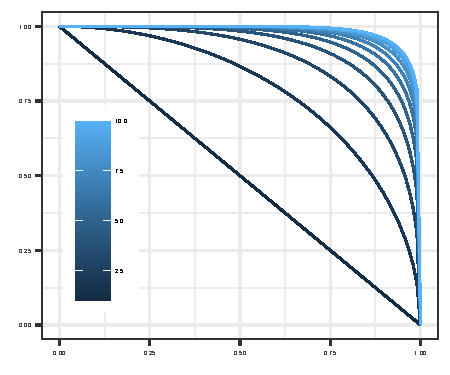
\includegraphics[width=0.12\textwidth]{images/p_sphere}
            ~
            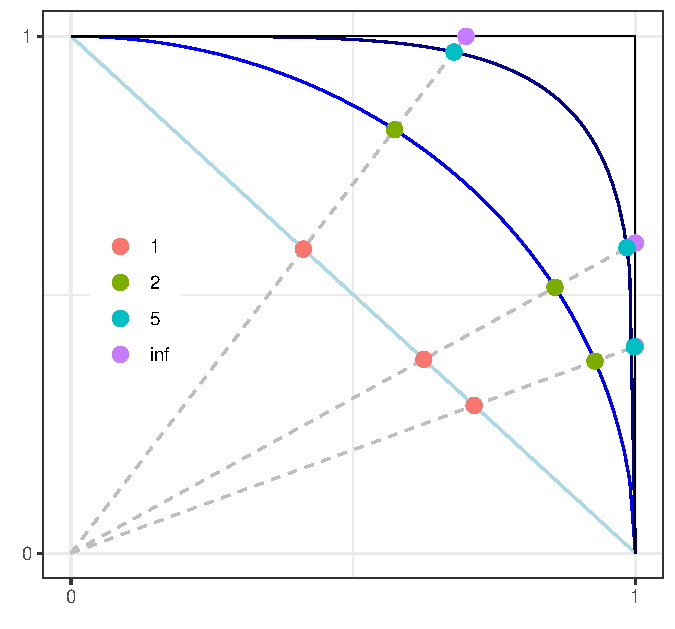
\includegraphics[width=0.12\textwidth]{images/p_project}
        \end{tikzfigure}
        \end{center}
    
        We recognize $\mathbb{S}_{\infty}^{d-1}$ as the positive orthant of the unit 
        hypersphere, under the $\mathcal{L}_{\infty}$ norm.  If we consider the 
        $\mathcal{L}_p$ norm, and then the $\mathbb{L}_{\infty}$ norm is expressed as the 
        limit of the $\mathcal{L}_p$ norm,
        \[
            \lVert \bm{s}\rVert_p = \left({\small\sum}_{\ell = 1}^d
                s_{\ell}^p\right)^{1/p},\;\;\;\;\;
            \lVert \bm{s}\rVert_{\infty} = 
            \lim\limits_{p\to\infty}\lVert \bm{s}\rVert_p = \bigvee_{\ell = 1}^d s_{\ell}.
        \]
        If we define $\mathbb{S}_{\infty}^{d-1}$ using this norm, then we consider it the 
        limit of of an expanding series of manifolds $\mathbb{S}_p^{d-1}$, the positive 
        orthant of the unit hypersphere under the $\mathcal{L}_p$ norm.  That is, for 
        $\bm{s}\in R_+^d$,
        \[ 
            \mathbb{S}_{\infty}^{d-1} = 
            \lim\limits_{p\to\infty}\left\lbrace \bm{x}\;\lVert \bm{x}\rVert_p =
            1\right\rbrace.\
        \]
        To establish a distribution on $\mathbb{S}_p^{d-1}$, we project a random vector from 
        $\mathbb{R}_+^d$ onto $\mathbb{S}_p^{d-1}$.  That is, for 
        $\mathbb{x}\in\mathbb{R}_+^d$, let 
        $\bm{y} = \frac{\bm{x}}{\lVert\bm{x}\rVert_p} \in \mathbb{S}_p^{d-1}$.  Then, by letting 
        $y_d = \left(1 - \sum_{\ell = 1}^{d-1}y_{\ell}^p\right)^{\frac{1}{p}}$, the
        transformation
        \[T(x_1,\ldots,x_d) = \left(\lVert \bm{x}\rVert p, \frac{x_1}{\lVert \bm{x}\rVert_p}, 
                \ldots, \frac{x_{d-1}}{\lVert \bm{x}\rVert_p}\right)\]
        is invertible with
        \[T^{-1}(r,y_1,\ldots,y_{d-1}) = 
            \left(ry_1,\ldots,ry_{d-1},r\left(1 - {\small\sum}_{\ell =
                1}^{d-1}y_{\ell}^p\right)^{\frac{1}{p}}\right).\]
        The determinant of the Jacobian of this transformation takes the form
        \[r^{d-1}\left[\left(1 - {\small\sum}_{\ell = 1}^{d-1}y_{\ell}^p\right)^{\frac{1}{p}} +
            {\small\sum}_{\ell = 1}^{d-1}y_{\ell}^p\left(1 - {\small\sum}_{\ell =
            1}^{d-1}y_{\ell}^p\right)^{\frac{1}{p} - 1}\right].\]
        Integrating out $r$ will yield a distribution on $\mathbb{S}_p^{d-1}$.
        With this transformation, we can project a density defined on $\mathbb{R}_+^{d-1}$ 
        onto $\mathbb{S}_{p}^{d-1}$ for any finite $p$.  Note that for $p=\infty$, the
        transformation is no longer differentiable.  Thus, our plan becomes to project 
        $\bm{V}$ onto a large but finite $p$, and assess model fidelity on $\mathbb{S}_{\infty}^{d-1}$
        }
        
    
    \block{Future Work in extreme analysis}
    {
    \begin{itemize}[noitemsep,nolistsep]
        \item Novelty detection in extremes using the projected gamma representation:
            \begin{itemize}[noitemsep,nolistsep]
                \item Inference in $\mathbb{S}_{\infty}^{d-1}$ introduces new possibilities of applications.  We hope to create an unsupervised--learning method of spotting anomalies---data that is not \emph{normal}.
            \end{itemize}
        \item A variational approach to Dirichlet process mixtures of projected gammas:
        \begin{itemize}[noitemsep,nolistsep]
            \item The log-normal centering distribution, and MCMC techniques for sampling DP's in general induce a great deal of computational complexity.  Our goal is combating this problem through a variational approach.
        \end{itemize}
    \end{itemize}
    }
\column{0.333}
\block{Projected Gamma Family \& DP mixtures thereof}
    {
    Given the form of the Jacobian, a natural distribution to consider in $\mathbb{R}_+^d$ is given by the product of 
    independent gamma distributions.  Let $\bm{X} \sim \prod_{\ell = 1}^d\text{Ga}(X_{\ell}\mid\alpha_{\ell},\beta_{\ell})$.  
    Using the transformation previously described, we have the joint density:
    \[
        \medmath{
        f(r,\bm{y}\mid\bm{\alpha},\bm{\beta}) = \prod_{\ell = 1}^d \left[ \frac{\beta_{\ell}^{\alpha_{\ell}}}{\Gamma(\alpha_{\ell}}
            (ry_{\ell})^{\alpha_{\ell} - 1}\exp\lbrace-\beta_{\ell}ry_{\ell}\rbrace\right]\times 
            r^{d-1}\left[\left(1 - \sum_{\ell = 1}^{d-1}y_{\ell}^p\right)^{\frac{1}{p}} +
            \sum_{\ell = 1}^{d-1}y_{\ell}^p\left(1 - \sum_{\ell = 1}^{d-1}y_{\ell}^p\right)^{\frac{1}{p} - 1}\right].
            }
    \]
    Integrating out $r$ yields the \emph{Projected Gamma} density,
    \[
        \medmath{
    \text{PG}\left(\bm{y}\mid\bm{\alpha},\bm{\beta}\right) = \prod_{\ell = 1}^d
        \left[\frac{\beta_{\ell}^{\alpha_{\ell}}}{\Gamma(\alpha_{\ell})}\right]
        \times \left[\left(1 - \sum_{\ell = 1}^{d-1}y_{\ell}^p\right)^{\frac{1}{p}} +
            \sum_{\ell = 1}^{d-1}y_{\ell}^p\left(1 - \sum_{\ell = 1}^{d-1}y_{\ell}^p\right)^{\frac{1}{p} - 1}\right]
        \times 
        \frac{\Gamma\left(\sum_{\ell = 1}^d\alpha_{\ell}\right)}{\left(\sum_{\ell = 1}^d
                \beta_{\ell}y_{\ell}\right)^{\sum_{\ell = 1}^d\alpha_{\ell}}}.
                }
    \]
    For identifiability, we fix $\beta_1 := 1$. This creates a moderately flexible distribution on
    $\mathbb{S}_p^{d-1}$ for any finite $p$. The projected gamma family is simple to specify and
    has very tractable computational properties. Thus, we use it as a building block to model the 
    angular distribution.  To build a flexible family of distributions on $\mathbb{S}_p^{d-1}$, we build a Dirichlet process mixture of the form
    \[
    \bm{y}_i\mid (\bm{\alpha}_i,\bm{\beta}_i) \sim \text{PG}(y_i\mid\bm{\alpha}_i,\bm{\beta}_i), \;\;\;\;
    (\alpha_i,\beta_i) \mid G \sim G, \;\;\;\; G \sim \text{DP}(\eta,G_0).
    \]
    We consider 4 options:
    \begin{itemize}
        \item \emph{Projected Gamma} (PG) vs \emph{Projected Restricted Gamma} (PRG) kernel distribution
        \item \emph{Product of Gammas} (--G) vs \emph{Multivariate Lognormal} (--LN) centering distribution
    \end{itemize}
    }
    \block{Results}{
    We conducted a simulation study to evaluate the performance of PG vs PRG, and ~--G vs ~--LN.
    
    \begin{tikzfigure}[Energy Score for recovering distribution of simulated data at a variety of columns, number of mixtures in generating distribution.]
        \centering 
        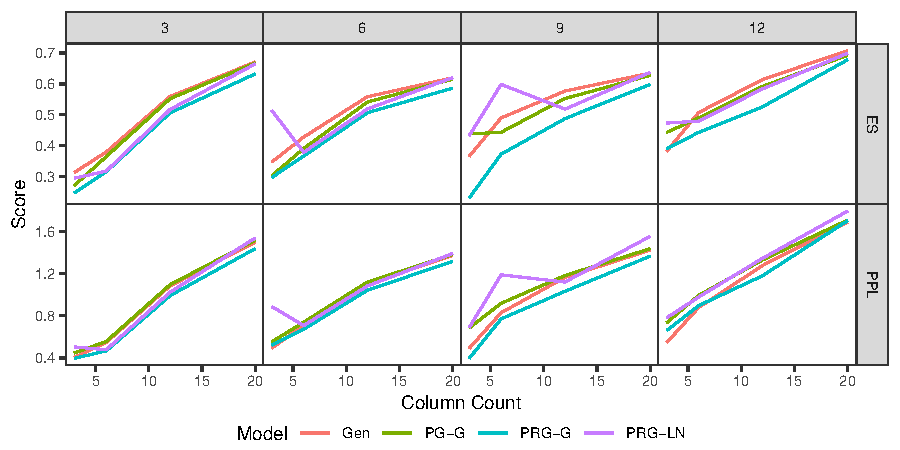
\includegraphics[width=0.25\textwidth,height=0.09\textwidth]{images/simulation_score}
    \end{tikzfigure}
    
    We interpret energy score formulated in this way as "lower is better".
    This indicates model fidelity was negatively affected by the
    additional flexibility offered in the unrestricted model (PG vs PRG).
    Interesting to note here is that the Log-normal model offers slightly worse
    performance as compared to the product of gammas. 
    
    We also tried the models against two datasets for the \emph{integrated vapor transport} (IVT).  This data captures the total amount of water vapor in the air in an atmospheric column, over a cell grid along California's coast.  ERA--Interim has 9 columns; and ERA5 has 43 columns.
    
    \begin{tikzfigure}[Energy Score for fitted models against IVT data]
        \centering
        \begin{tabular}{ccc}
        \toprule
        Model   & ERA--Interim  & ERA--5\\
        \midrule
        PRG--G  & {\bf 0.172}   & 0.751       \\
        PRG--LN & 0.173         & {\bf 0.714} \\
        PG--G   & 0.426         & 1.169       \\
        PG--LN  & 0.294         & 0.799       \\
        \bottomrule
        \end{tabular}
    \end{tikzfigure}
    
    We see a slight reversal here, as compared to the simulation, where the log-normal models are preferred for the high-dimensional data.
    }
    
\end{columns}












% \block{Angular Distributions}{Here, \blindtext \vspace{4cm}}
%     \note[
%         targetoffsetx=-9cm, 
%         targetoffsety=-6.5cm, 
%         width=0.4\linewidth
%         ]
%         {e-mail \texttt{welcome@overleaf.com}}
% \begin{columns}
%     \column{0.5}
%     \block{A figure}
%     {
%         \begin{tikzfigure}
%             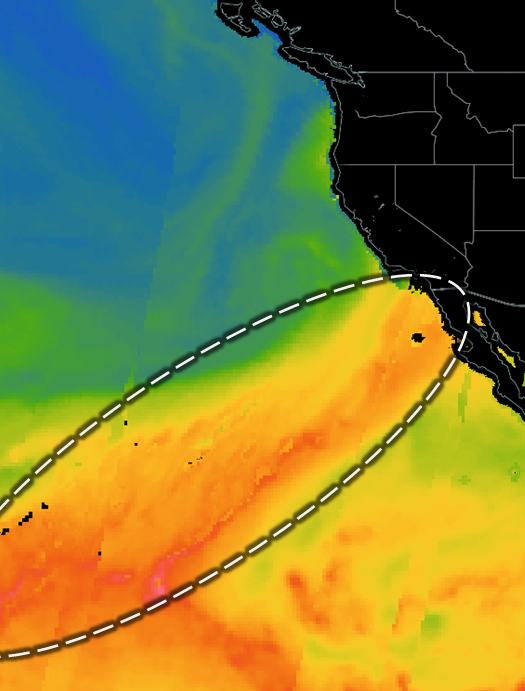
\includegraphics[width=0.4\textwidth]{images/ar}
%         \end{tikzfigure}
%     }
%     \column{0.5}
%     \block{Description of the figure}{\blindtext}
% \end{columns}

\end{document}
